\documentclass{beamer}
\usepackage[utf8]{inputenc}

\usetheme{Madrid}
\usecolortheme{default}
\usepackage{amsmath,amssymb,amsfonts,amsthm}
\usepackage{txfonts}
\usepackage{tkz-euclide}
\usepackage{listings}
\usepackage{adjustbox}
\usepackage{array}
\usepackage{tabularx}
\usepackage{gvv}
\usepackage{lmodern}
\usepackage{circuitikz}
\usepackage{tikz}
\usepackage{graphicx}

\setbeamertemplate{page number in head/foot}[totalframenumber]

\title{4.2.4}
\date{\today}
\author{EE25BTECH11001 - Aarush Dilawri}

\begin{document}

\frame{\titlepage}

\begin{frame}{Question}
\textbf{Question:} \\
Find the direction and normal vector for the line 
\begin{align}
x = 3y
\end{align}
\end{frame}

\begin{frame}{Solution}
The line can be written as: 
\begin{align}
x - 3y =0
\end{align}

This equation can be expressed in terms of matrices:\\
Let
\begin{align}
\vec{x} = \myvec{x \\ y}
\end{align}
\begin{align}
\vec{n^T} = \myvec{1 & -3}
\end{align}
\begin{align}
c = 0
\end{align}

The line equation can be written as:
\begin{align}
\vec{n^T}  \vec{x} = c
\end{align}

Where $\vec{n}$ is the normal vector of the given line
\end{frame}

\begin{frame}{Direction Vector}
The direction vector of the line can be found by observing the normal vector.
\begin{align}
\vec{m} = \myvec{3 \\ 1}
\end{align}

This is true because if the director vector is represented as 
\begin{align}
\vec{m}  = \myvec{1 \\ m}    
\end{align}
then the normal vector can be represented as 
\begin{align}
\vec{n} = \myvec{-m \\ 1}
\end{align}

This can be verified by the following equation:
\begin{align}
\vec{n^T}\vec{m} = 0
\end{align}
\end{frame}
\begin{frame}{Conclusion}

\begin{align}
\myvec{1 & -3}\myvec{3 \\ 1} = 0
\end{align}


The normal vector of the line is 
\begin{align}
\vec{n} = \myvec{1 \\ -3}
\end{align}

The director vector of the line is 
\begin{align}
\vec{m} = \myvec{3 \\ 1}
\end{align}


\end{frame}

\begin{frame}{Figure}
From the figure, it is clearly verified that the theoretical solution matches with the computational solution.
\begin{figure}[h!]
    \centering
    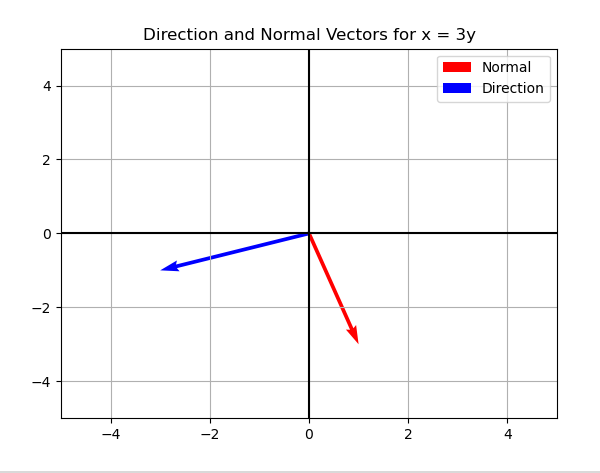
\includegraphics[height=0.5\textheight, keepaspectratio]{figs/fig.png}
    %\caption{Direction and Normal Vectors}
\end{figure}
\end{frame}


% ---------- C CODE ----------
\begin{frame}[fragile]{C Code (code.c)}
\begin{lstlisting}[language=C]
#include <stdio.h>

// Generalized dot product of two n-dimensional vectors
int dot_product(const int* a, const int* b, int n) {
    int sum = 0;
    for(int i = 0; i < n; i++) {
        sum += a[i] * b[i];
    }
    return sum;
}

// Check if two n-dimensional vectors are orthogonal
int is_orthogonal(const int* a, const int* b, int n) {
    return dot_product(a, b, n) == 0;
}

\end{lstlisting}
\end{frame}
\begin{frame}[fragile]{C Code (code.c)}
\begin{lstlisting}[language=C]
// Compute normal vector of a 2D line Ax + By = C
// Returns result in nvec array (size 2)
void normal_vector(int A, int B, int* nvec) {
    nvec[0] = A;
    nvec[1] = B;
}

// Compute direction vector of a 2D line Ax + By = C
// Returns result in dvec array (size 2)
void direction_vector(int A, int B, int* dvec) {
    dvec[0] = B;
    dvec[1] = -A;
}
\end{lstlisting}
\end{frame}
\begin{frame}[fragile]{Python Code (code.py)}
\begin{lstlisting}[language=Python]
import numpy as np
import matplotlib.pyplot as plt

# Generalized dot product
def dot_product(a, b):
    if len(a) != len(b):
        raise ValueError("Vectors must have same length")
    return sum(a[i]*b[i] for i in range(len(a)))

# Check orthogonality
def is_orthogonal(a, b):
    return dot_product(a, b) == 0

# Normal and direction vectors for a 2D line Ax + By = C
def normal_vector(A, B):
    return np.array([A, B])
\end{lstlisting}
\end{frame}

\begin{frame}[fragile]{Python Code (code.py)}
\begin{lstlisting}[language=Python]
def direction_vector(A, B):
    return np.array([B, -A])

# Example: x = 3y => 1*x - 3*y = 0
A, B = 1, -3
nvec = normal_vector(A, B)
dvec = direction_vector(A, B)

print("Normal vector:", nvec)
print("Direction vector:", dvec)
print("Orthogonal check:", is_orthogonal(nvec, dvec))

# Plotting
origin = np.array([[0,0]])
\end{lstlisting}
\end{frame}
\begin{frame}[fragile]{Python Code (code.py)}
\begin{lstlisting}[language=Python]
plt.quiver(*origin.T, nvec[0], nvec[1], color='r', scale=1, scale_units='xy', angles='xy', label='Normal')
plt.quiver(*origin.T, dvec[0], dvec[1], color='b', scale=1, scale_units='xy', angles='xy', label='Direction')

plt.xlim(-5,5)
plt.ylim(-5,5)
plt.grid(True)
plt.axhline(0, color='black')
plt.axvline(0, color='black')
plt.legend()
plt.title('Direction and Normal Vectors for x = 3y')
plt.show()
\end{lstlisting}
\end{frame}

\begin{frame}[fragile]{Python Code (nativecode.py)}
\begin{lstlisting}[language=Python]
import ctypes
import numpy as np
import matplotlib.pyplot as plt

# Load shared library
lib = ctypes.CDLL('./code.so')

# Set argument and return types
lib.dot_product.argtypes = [ctypes.POINTER(ctypes.c_int), ctypes.POINTER(ctypes.c_int), ctypes.c_int]
lib.dot_product.restype = ctypes.c_int

lib.is_orthogonal.argtypes = [ctypes.POINTER(ctypes.c_int), ctypes.POINTER(ctypes.c_int), ctypes.c_int]
lib.is_orthogonal.restype = ctypes.c_int

lib.normal_vector.argtypes = [ctypes.c_int, ctypes.c_int, ctypes.POINTER(ctypes.c_int)]
lib.direction_vector.argtypes = [ctypes.c_int, ctypes.c_int, ctypes.POINTER(ctypes.c_int)]
\end{lstlisting}
\end{frame}
\begin{frame}[fragile]{Python Code (nativecode.py)}
\begin{lstlisting}[language=Python]
# Prepare arrays for 2D vectors
nvec = (ctypes.c_int * 2)()
dvec = (ctypes.c_int * 2)()

# Line: x = 3y => 1*x - 3*y = 0
A, B = 1, -3

lib.normal_vector(A, B, nvec)
lib.direction_vector(A, B, dvec)

print("Normal vector:", list(nvec))
print("Direction vector:", list(dvec))

# Plot vectors
origin = np.array([[0,0]])
\end{lstlisting}
\end{frame}
\begin{frame}[fragile]{Python Code (nativecode.py)}
\begin{lstlisting}[language=Python]
plt.quiver(*origin.T, nvec[0], nvec[1], color='r', scale=1, scale_units='xy', angles='xy', label='Normal')
plt.quiver(*origin.T, dvec[0], dvec[1], color='b', scale=1, scale_units='xy', angles='xy', label='Direction')

plt.xlim(-5,5)
plt.ylim(-5,5)
plt.grid(True)
plt.axhline(0, color='black')
plt.axvline(0, color='black')
plt.legend()
plt.title('Direction and Normal Vectors for x = 3y')
plt.show()
\end{lstlisting}
\end{frame}
\end{document}